\documentclass{article}
\setlength{\parskip}{0pt} % esp. entre parrafos
\setlength{\parindent}{20pt} % esp. al inicio de un parrafo
\usepackage{amsmath} % mates
\usepackage{listings}
\usepackage{xcolor}
\usepackage[sort&compress,numbers]{natbib} % referencias
\usepackage{url} % que las URLs se vean lindas
\usepackage[top=10mm,left=20mm,right=20mm,bottom=25mm]{geometry} % \textbf{\textbf{}}margenes
\usepackage{hyperref} % ligas de URLs
\usepackage{graphicx} % poner figuras
\usepackage{caption}
\usepackage{subcaption}
\usepackage[spanish]{babel} % otros idiomas
\hypersetup{
    colorlinks=true,
    linkcolor=blue,
    filecolor=blue,      
    urlcolor=blue,
}
\renewcommand{\lstlistingname}{C\'odigo}
\definecolor{codegreen}{rgb}{0,0.6,0}
\definecolor{codegray}{rgb}{0.5,0.5,0.5}
\definecolor{codepurple}{rgb}{0.58,0,0.82}
\definecolor{backcolour}{rgb}{0.95,0.95,0.92}
\lstdefinestyle{mystyle}{
    backgroundcolor=\color{backcolour},   
    commentstyle=\color{codegreen},
    keywordstyle=\color{magenta},
    numberstyle=\tiny\color{codegray},
    stringstyle=\color{codepurple},
    basicstyle=\ttfamily\footnotesize,
    breakatwhitespace=false,         
    breaklines=true,                 
    keepspaces=true,                 
    numbers=left,                    
    numbersep=5pt,                  
    showspaces=false,                
    showstringspaces=false,
    showtabs=false,                  
    tabsize=2
}
\lstset{style=mystyle}

\title{Reporte 4:\\Diagramas de Voronoi}
\author{Jorge Torres}
\date{\today}

\begin{document}

\maketitle

\section{Objetivo}
En esta pr\'actica se genera un conjunto de celdas de Voronoi, tambi\'en llamadas mosaicos de Dirichlet, con el m\'etodo computacional descrito por P. J. Green y R. Sibson \cite{green}. Se determina el efecto que tiene el variar la densidad de semillas en cinco niveles ($k = 25, 50, 75, 100, 125$), en la probabilidad de que una segunda grieta llegue a tocar una primera, es decir, fracturando la pieza dos veces con posiciones iniciales generadas independientemente al azar, sobre varias réplicas. Se analizan los resultados y se visualizan en la secci\'on \ref{res}.

\section{Desarrollo}
El c\'odigo que se describe en esta pr\'actica est\'a basado en el \href{https://github.com/satuelisa/Simulation/blob/master/VoronoiDiagrams/fracture.py}{desarrollado} por E. Schaeffer \cite{elisa1}, y se puede encontrar en su totalidad en el \href{https://github.com/FeroxDeitas/Simulacion-Nano/blob/main/Tareas/P4/voronoi.py}{repositorio} de J. Torres en GitHub.\\

El primer paso consiste en definir los par\'ametros iniciales de operaci\'on, a partir de los cuales se generan las celdas de Voronoi. Estos consisten en un tamaño de matriz de 100, cinco niveles para la densidad inicial de semillas y 200 repeticiones del experimento para cada una de ellas (ver c\'odigo \ref{codigo1}).

\begin{lstlisting}[caption=Par\'ametros, label=codigo1, language=Python]
n = 100
seed = [25, 50, 75, 100, 125]
runs = 200
\end{lstlisting}

En el c\'odigo \ref{codigo2} se define la funci\'on \texttt{creacion()}, en donde colocan las semillas en el plano de manera aleatoria, mientras que con la funci\'on \texttt{celda()} se determinan las distancias euclideanas m\'as cercanas a cada semilla, definiendo as\'i la celda de Voronoi para dicha semilla.

\begin{lstlisting}[caption=Ubicaci\'on de semillas y celdas, label=codigo2, language=Python]
def creacion():
    semillas = []
    for s in range(k):
        while True:
            x, y = randint(0, n - 1), randint(0, n - 1)
            if (x, y) not in semillas:
                semillas.append((x, y))
                break
    return semillas

def celda(pos):
    if pos in semillas:
        return semillas.index(pos)
    x, y = pos % n, pos // n
    cercano = None
    menor = n * sqrt(2)
    for i in range(k):
        (xs, ys) = semillas[i]
        dx, dy = x - xs, y - ys
        dist = sqrt(dx**2 + dy**2)
        if dist < menor:
            cercano, menor = i, dist
    return cercano
\end{lstlisting}

Al tener las celdas definidas, se puede proseguir a determinar, de manera aleatoria, la posici\'on inicial de la grieta con la funci\'on \texttt{inicio()} descrita en el c\'odigo \ref{codigo3}.

\begin{lstlisting}[caption= Ubicaci\'on inicial de la grieta, label=codigo3, language=Python]
def inicio():
    direccion = randint(0, 3)
    if direccion == 0:
        return (0, randint(0, n - 1))
    elif direccion == 1:
        return (randint(0, n - 1), 0)
    elif direccion == 2:
        return (randint(0, n - 1), n - 1)
    else:
        return (n - 1, randint(0, n - 1))
\end{lstlisting}

Para propagar la grieta se tiene en cuenta que es m\'as probable que se propague a lo largo de una frontera de celda, mientras que en el interior la probabilidad va disminuyendo gradualmente. En el c\'odigo \ref{codigo4} se propaga una grieta en color negro hasta que toca un borde o hasta que le es demasiado dif\'icil seguir propag\'andose al interior de una celda.

\begin{lstlisting}[caption=Propagaci\'on de la primera grieta, label=codigo4, language=Python]
def propaga_n():
    prob, dificil = 0.9, 0.8
    grieta_n = voronoi.copy()
    g = grieta_n.load()
    (xn, yn) = inicio()
    negro = (0, 0, 0)
    while True:
        g[xn, yn] = negro
        frontera, interior = [], []
        for v in vecinos:
            (dx, dy) = v
            vx, vy = xn + dx, yn + dy
            if vx >= 0 and vx < n and vy >= 0 and vy < n:
               if g[vx, vy] != negro:
                   if vor[vx, vy] == vor[xn, yn]:
                       interior.append(v)
                   else:
                       frontera.append(v)
        elegido = None
        if len(frontera) > 0:
            elegido = choice(frontera)
            prob = 1
        elif len(interior) > 0:
            elegido = choice(interior)
            prob *= dificil
        if elegido is not None:
            (dx, dy) = elegido
            xn, yn = xn + dx, yn + dy
        else:
            break
    return grieta_n
\end{lstlisting}

Se puede generar una segunda grieta (en color blanco) con la funci\'on \texttt{inicio()} del c\'odigo \ref{codigo3}. \'Esta se propagar\'ia de la misma manera que la primera, con la excepci\'on de que se detiene por completo al hacer contacto con la primera grieta. Este comportamiento se puede observar en el c\'odigo \ref{codigo5}.

\begin{lstlisting}[caption=Propagaci\'on de la segunda grieta, label=codigo5, language=Python]
def propaga_b():
    prob, dificil = 0.9, 0.8
    grieta_b = propaga_n()
    g = grieta_b.load()
    (xb, yb) = inicio()
    blanco = (255, 255, 255)
    negro = (0, 0, 0)
    while True:
        g[xb, yb] = blanco
        frontera, interior = [], []
        for v in vecinos:
            (dx, dy) = v
            vx, vy = xb + dx, yb + dy
            if vx >= 0 and vx < n and vy >= 0 and vy < n:
               if g[vx, vy] != blanco:
                   if vor[vx, vy] == vor[xb, yb]:
                       interior.append(v)
                   else:
                       frontera.append(v)
        elegido = None
        if len(frontera) > 0:
            elegido = choice(frontera)
            prob = 1
        elif len(interior) > 0:
            elegido = choice(interior)
            prob *= dificil
        if elegido is not None:
            (dx, dy) = elegido
            xb, yb = xb + dx, yb + dy
            if g[xb, yb] == negro:
                tocaron.append(1)
                break
        else:
            break
    return grieta_b
\end{lstlisting}

En el c\'odigo \ref{codigo6} se inicializan las funciones descritas anteriormente. El experimento se repite 200 veces para cada una de las densidades iniciales de semillas. Se lleva un conteo de las veces que se tocaron y se calcula la probabilidad de que se toquen basada en esos resultados utilizando la ecuaci\'on \ref{eq1},

\begin{equation}\label{eq1}
    P = \frac{N_T}{R} \times 100
\end{equation}
donde $N_T$ es la cantidad de veces que se tocaron y $R$ es la cantidad de iteraciones.
\begin{lstlisting}[caption=Iteraciones del experimento, label=codigo6, language=Python]
for k in seed:
    tocaron = []
    for r in range(runs):
        semillas = creacion()
        celdas = [celda(i) for i in range(n * n)]
        voronoi = Image.new('RGB', (n, n))
        vor = voronoi.load()
        c = sns.color_palette("Set3", k).as_hex()
        for i in range(n * n):
            vor[i % n, i // n] = ImageColor.getrgb(c[celdas.pop(0)])
        limite, vecinos = n, []
        for dx in range(-1, 2):
            for dy in range(-1, 2):
                if dx != 0 or dy != 0:
                    vecinos.append((dx, dy))
        propaga_b()
    pr = (len(tocaron)/runs)*100
    resultado.append(pr)
\end{lstlisting}
\section{Resultados}\label{res}
Para una mejor visualizaci\'on de la generaci\'on de las celdas y las grietas, en la figura \ref{grietas} se exponen un par de ejemplos de \'estas. Uno donde las grietas no se tocan (figura \ref{fig:notocan}), y otro donde las grietas se tocan (figura \ref{fig:tocan}). Por otro lado, en la figura \ref{prob} se muestran las probabilidades calculadas de que las grietas se toquen para los cinco distintos niveles de densidad de semillas.
\begin{figure}
     \centering
     \begin{subfigure}[b]{0.49\textwidth}
         \centering
         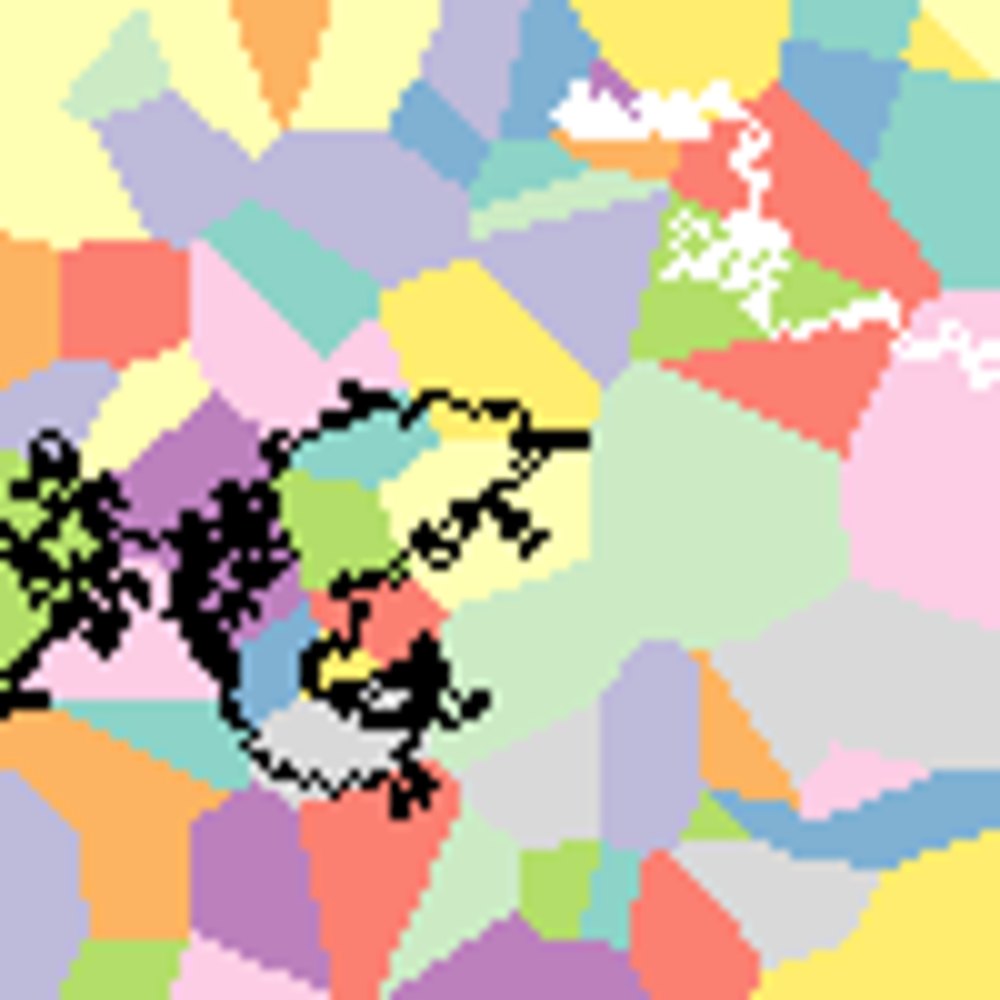
\includegraphics[width=\textwidth]{p4pgbn_75_5.png}
         \caption{Las grietas no se tocan.}
         \label{fig:notocan}
     \end{subfigure}
     \begin{subfigure}[b]{0.49\textwidth}
         \centering
         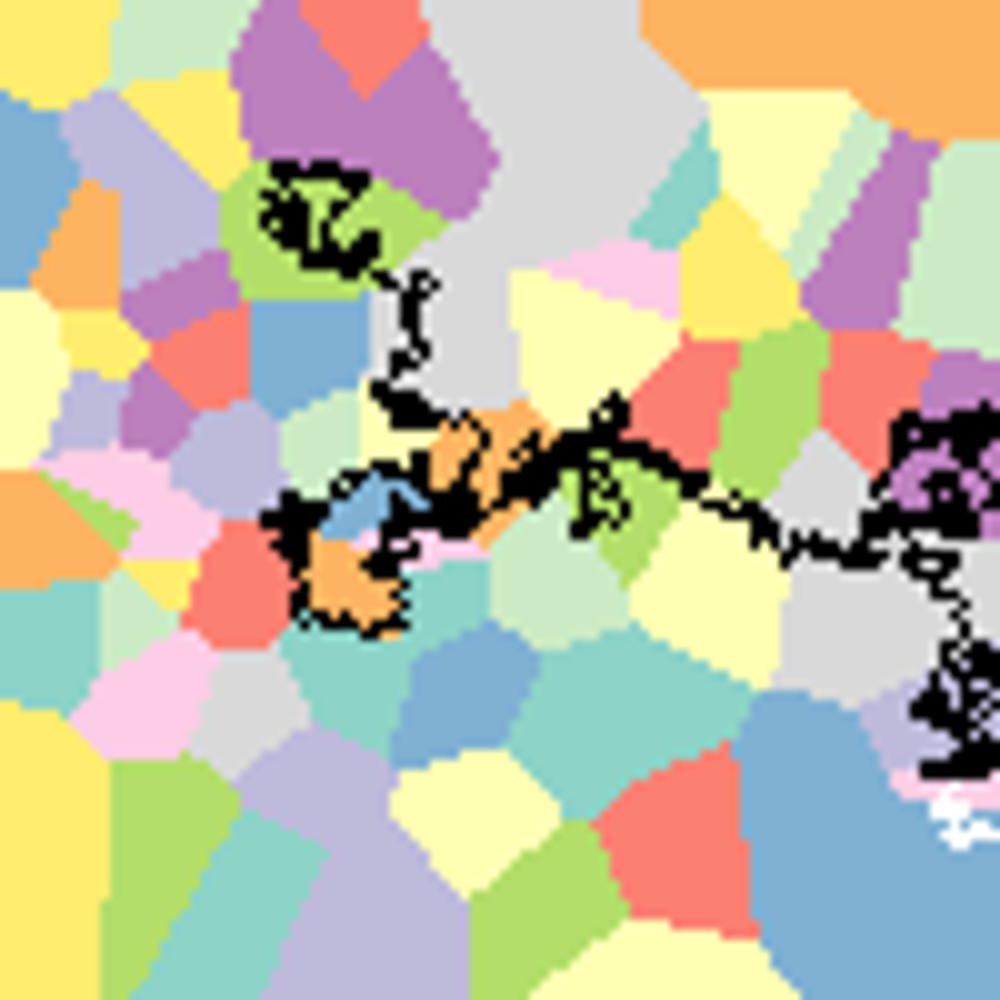
\includegraphics[width=\textwidth]{p4pgbn_75_8.png}
         \caption{Las grietas se tocan.}
         \label{fig:tocan}
     \end{subfigure}
     \caption{Ejemplos de grietas.}
     \label{grietas}
\end{figure}

\begin{figure}
    \centering
    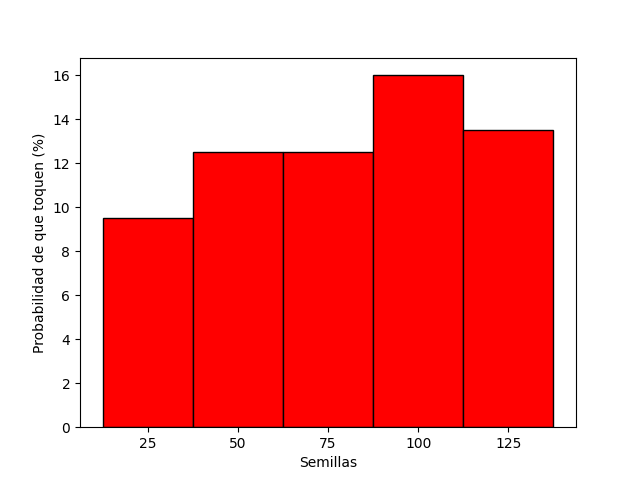
\includegraphics[width=\textwidth]{Voronoi.png}
    \caption{Probabilidades de que las grietas se toquen para los cinco niveles de densidad de semillas.}
    \label{prob}
\end{figure}
\section{Conclusiones}\label{con}
Observando la gr\'afica de la figura \ref{prob}, podr\'ia aparentar que la probabilidad de que las grietas se toquen aumenta conforme se aumenta tambi\'en la densidad de semillas. Debido a la naturaleza aleatoria del sistema, ser\'ia dif\'icil decir con certeza el por qu\'e esto es as\'i, sin embargo podr\'ia deberse a que la cantidad de fronteras aumenta con la cantidad de semillas, adem\'as de que el tamaño promedio de celda disminuye, lo cual ser\'ia propicio para que las grietas coincidan en un lugar. Sin embargo, la probabilidad disminuye ligeramente en el \'ultimo nivel, lo cual hace pensar que existe un l\'imite para la propagaci\'on de las grietas. La determinaci\'on de dicho l\'imite se encuentra fuera del rango de estudio de \'esta pr\'actica.
\bibliography{tarea_4}
\bibliographystyle{plainnat}
\end{document}
